\chapter{Inżynieria danych eksperymentalnych i testowe szablony modeli}
\section{Omówienie danych eksperymentalnych}
	
	W celu zestawienia funkcjonalnego bibliotek uczenia maszynowego w języku C++ i przedstawienia przykładów konieczne było wybranie danych eksperymentalnych możliwych do wykorzystania jako porównawczy punkt odniesienia. Jako w/w dane wybrano bazę dotyczącą diagnostyki raka piersi, w której zamieszczono wyniki obrazowania określone w sposób liczbowy. Dane mają następującą strukturę:
	
	\begin{enumerate}
		\item [1)] ID - numer identyfikacyjny pacjentki;
		\item [2)] Diagnosis [\textit{Malignant - M} / \textit{Benign - B}] - charakter nowotworu, \textbf{zmienna odpowiedzi};
		\item [3)] Dane klasyfikujące:
			\begin{enumerate}
				\item [a)] \textit{Radius} - średnica guza;
				\item [b)] \textit{Texture} - tekstura guza;
				\item [c)] \textit{Perimeter} - obwód guza;
				\item [d)] \textit{Area} - pole guza;
				\item [e)] \textit{Smoothness} - gładkość, miara lokalnych różnic w promieniu guza;
				\item [f)] \textit{Compactness} - zwartość, wykorzystywana do oceny stadium guza;
				\item [g)] \textit{Concavity} - stopień wklęsłości miejsc guza;
				\item [h)] \textit{Concave points} - punkty wklęsłości guza;
				\item [i)] \textit{Symmetry} - symetria guza, pomagająca w ocenie charakteru przyrostu guza.
				\item [j)] \textit{Fractal dimention (,,coastline approximation'' - 1)} - wymiar fraktalny pozwalający na ilościowy opis złożoności komórek nerwowych, umożliwiający stwierdzenie nowotworzenia się zbioru komórek.
			\end{enumerate}
	\end{enumerate}
	
	Dla każdej ze zmiennych odpowiedzi została zebrana średnia wartość, odcyhelenie standardowe oraz średnia trzech największych pomiarów, gdzie każdy zestaw ustawiony jest sekwencyjnie (np. kolumna 3 - średni promień, kolumna 12 - odchylenie standardowe promienia, kolumna 22 - średnia trzech największych pomiarów promienia). Każda ze zmiennych ma charakter ciągły.
	
\section{Charakterystyka i przetwarzenie danych}

	W celu przeprowadzenia procesu uczenia maszynowego, jednym z najistotniejszych kroków jakie należy podjąć jest wstępne zaznajomienie się z zestawem danych i jego analiza pod kątem rozkładu poszczególnych zmiennych oraz prawdopodobieństw. W tym celu wykorzystane zostało oprogramowanie JMP. 

	\subsection{Analiza rozkładu danych}
	
	\begin{figure}[!ht]
		\centering
		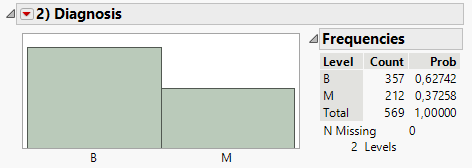
\includegraphics[width=0.8\linewidth]{Rysunki/Rozdzial2/diagnosis_distribution}
		\caption{Histogram rozkładu zmiennej odpowiedzi}
		\label{fig:diagnosisdistribution}
	\end{figure}
	
	\begin{figure}[!ht]
		\centering
		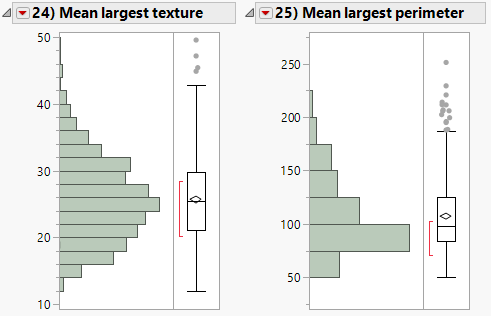
\includegraphics[width=0.7\linewidth]{Rysunki/Rozdzial2/variable_distribution}
		\caption{Przykłady histogramów zmiennych decyzyjnych}
		\label{fig:variabledistribution}
	\end{figure}
	
	
	Proces analizy rozkładu rozpoczęty został od przyjrzenia się zmiennej odpowiedzi (\textit{Diagnosis}). Rysunek 3.1 przedstawia uzyskany histogram, wraz z tabelą określającą ilość obserwacji danej klasy i współczynnik prawdopodobieństwa przynależności odpowiedzi do danej klasy. Zauważyć można, że dla użytego zestawu danych ilość zarejestrowano 357 obserwacji łagodnego raka piersi, a jego prawdopodobieństwo przynależności do klasy \textit{Benign} wynosi $\approx$ 62,7\%, natomiast do klasy \textit{Malignant} przynależało 212 obserwacji z prawodpodobieństwem $\approx$ 37,3\%.
		
	Podczas analizy histogramów zmiennych decyzyjnych, stwierdzono że znaczna ilość ma charakter prawostronnie skośny oraz występują dla nich obserwacje odstające, o czym informuje znajdujący się po prawej stronie histogramu wykres okienkowy (ang. \textit{box graph}), co przedstawiono na rysunku 3.2. Wyjątkiem okazała się zmienna \textit{Mean Largest Concave Points}), która mimo lekkiej skośności, okazała się nie posiadać obserwacji odstających. Na podstawie tych informacji stwierdzono, że aby przygotować dane w odpowiedni sposób do procesu uczenia należy przeprowadzić ich czyszczenie oraz normalizację rozkładu.
	
	\subsection{Czyszczenie i normalizacja rozkładu danych}
	
	Na pełny zestaw danych składa się 569 obserwacji. Podczas wstępnej analizy nie stwierdzono istnienia brakujących wartości, w związku z czym głównym problemem okazały się obserwacje odstające oraz skośności rozkładu. Do analizy obserwacji odstających wykorzystano wykresy okienkowe, gdzie oś Y reprezentowała zmienną odpowiedzi, natomiast oś X czyszczoną zmienną decyzyjną. Przykładowy wykres został przedstawiony na rysunku 3.3. Ze względu na bardzo małą ilość obserwacji zdecydowano się rozpocząć proces przystosowywania danych do uczenia poprzez normalizację ich rozkładu, aby zminimalizować lub wyeliminować konieczność usunięcia danych odstających. 
	
	\begin{figure}[!ht]
		\centering
		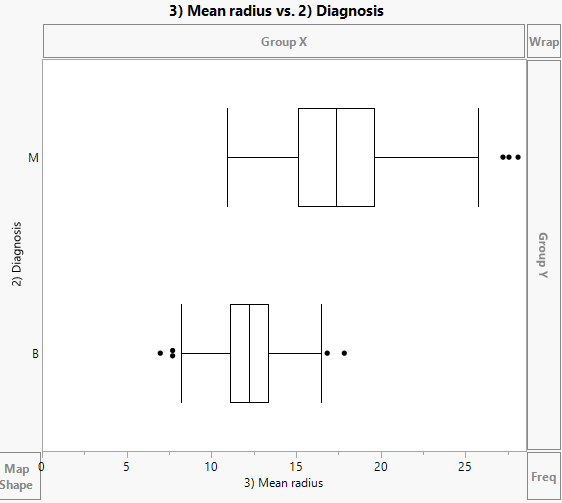
\includegraphics[width=0.7\linewidth]{Rysunki/Rozdzial2/box_graph}
		\caption{Przykład analizy obserwacji odstających dla poszczególnych klas zmiennej odpowiedzi}
		\label{fig:boxgraph}
	\end{figure}

	\newpage
	
	W pierwszym podejściu zdecydowano się na zastosowanie transformacji logarytmicznej dla wszystkich zmiennych decyzyjnych i porównanie charakterystyk uzyskanych rozkładów z oryginalnymi. Zmienna \textit{Mean largest concave points} okazała się posiadać rozkład bardzo zbliżony do standardowego, w związku z czym wyłączono ją z dalszej analizy normalizacji.Przykładowe wyniki przedstawiono na rysunkach 3.4 oraz 3.5. Transformacja ta okazała się skutecznym rozwiązaniem jedynie dla następujących zmiennych:
	
	\begin{enumerate}
		\item \textit{Mean radius};
		\item \textit{Mean texture};
		\item \textit{Mean perimeter},
		\item \textit{Mean area};
		\item \textit{Mean smoothness};
		\item \textit{Mean symmetry};
		\item \textit{Std err texture};
		\item \textit{Std err smoothness};
		\item \textit{Std err compactness};
		\item \textit{Std err concave points};
		\item \textit{Mean largest texture};
		\item \textit{Mean largest smoothness};
		\item \textit{Mean largest compactness}.
	\end{enumerate}

	\begin{figure}[!ht]
		\centering
		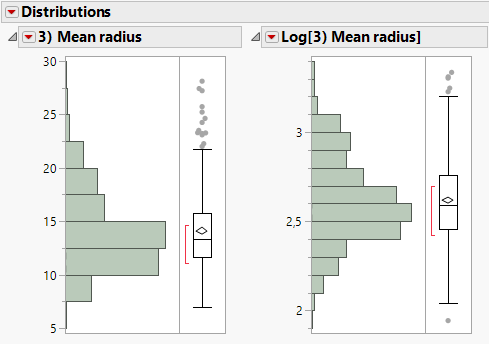
\includegraphics[width=0.7\linewidth]{Rysunki/Rozdzial3/log}
		\caption{Porównanie rozkładu danych przed i po transformacji logarytmicznej.}
		\label{fig:log}
	\end{figure}
	
	\newpage

	W drugim kroku podjęto próbę wykorzystania transformacji pierwiastkiem sześciennym dla pozostałych zmiennych decyzyjych, ze względu na jej skuteczność dla danych o rozkładzie prawoskośnym. Rysunek 3.6. przedstawia porównanie rozkładu zmiennej \textit{Mean concavity} przed i po transfromacji pierwiastkiem sześciennym. Pomyślnie znormalizowano rozkład następujących zmiennych:
	
	\begin{enumerate}
		\item \textit{Mean compactness};
		\item \textit{Mean concavity};
		\item \textit{Mean concave points};
		\item \textit{Std err concavity};
		\item \textit{Mean largest radius};
		\item \textit{Mean largest perimeter};
		\item \textit{Mean largest concavity};
		\item \textit{Mean largest symmetry}.
	\end{enumerate} 

\begin{figure}[!ht]
	\centering
	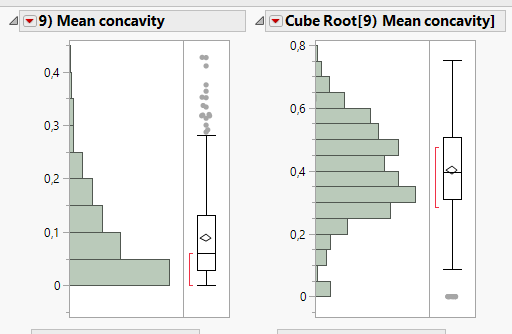
\includegraphics[width=0.7\linewidth]{Rysunki/Rozdzial3/cube_root}
	\caption{Porównanie rozkładów danych przed i po zastosowaniu transformacji pierwiastkiem sześciennym.}
	\label{fig:cuberoot}
\end{figure}

	

\section{Szablony docelowych modeli dla zadanych danych eksperymentalnych}

Ze względu na dychotomiczny charakter zmiennej odpowiedzi, wybrany został przedstawiony poniżej zestaw metod dla których wykonano i przedstawiono testy praktyczne. Szablony struktury rozwiązań, takie jak np. wybór zmiennych uczestniczących w procesie uczenia, lub struktura sieci neuronowej zostały ustalone w sposób empiryczny z wykorzystaniem programu do uczenia maszynowego JMP. 

\subsection{Regresja logistyczna}

\subsection{Głęboka sieć neuronowa}

\subsection{Maszyna wektorów nośnych}